\documentclass[border=4pt]{standalone}
\usepackage{lmodern}
\usepackage{amsmath,amssymb}
\usepackage{pgfplots}
\pgfplotsset{compat=1.18}
\begin{document}
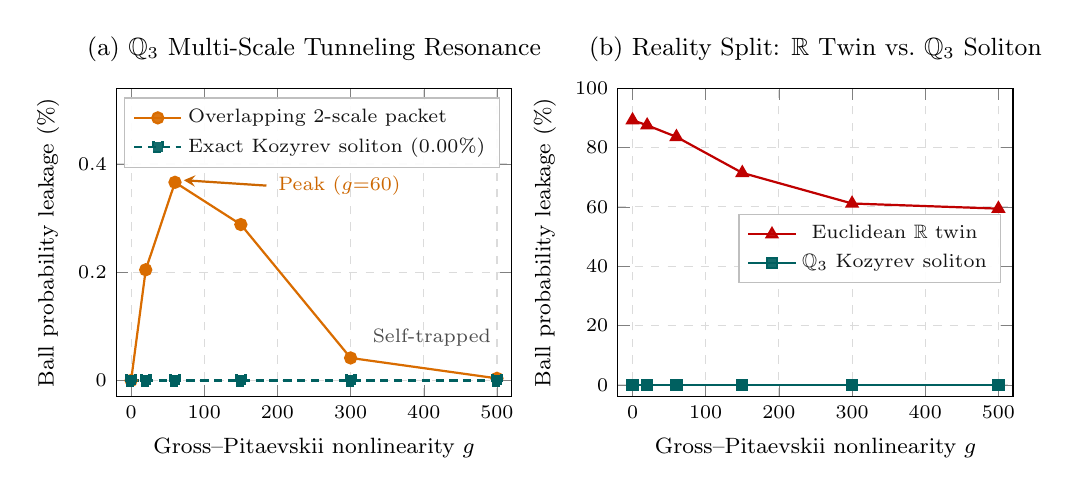
\begin{tikzpicture}
\begin{axis}[
  name=leftplot,
  width=6.6cm,
  height=5.5cm,
  title={\small (a) $\mathbb{Q}_3$ Multi-Scale Tunneling Resonance},
  xlabel={Gross--Pitaevskii nonlinearity $g$},
  ylabel={Ball probability leakage (\%)},
  xmin=-20, xmax=520,
  ymin=-0.03, ymax=0.54,
  grid=major,
  grid style={dashed, gray!28},
  legend pos=north east,
  legend cell align=left,
  legend style={font=\scriptsize, fill=white, fill opacity=0.92, draw=gray!50},
  label style={font=\footnotesize},
  tick label style={font=\scriptsize},
]
  \addplot[color=orange!85!black, thick, mark=*, mark size=2.0pt] coordinates { (0, 0.0000) (20, 0.2045) (60, 0.3661) (150, 0.2881) (300, 0.0416) (500, 0.0039) };
  \addlegendentry{Overlapping 2-scale packet}
  \addplot[color=teal!75!black, thick, densely dashed, mark=square*, mark size=1.8pt] coordinates { (0, 0.000000) (20, 0.000000) (60, 0.000000) (150, 0.000000) (300, 0.000000) (500, 0.000000) };
  \addlegendentry{Exact Kozyrev soliton ($0.00\%$)}
  \draw[->, >=stealth, orange!80!black, thick] (axis cs:185, 0.36) -- (axis cs:72, 0.37);
  \node[anchor=west, font=\scriptsize, text=orange!80!black] at (axis cs:188, 0.36) {Peak ($g{=}60$)};
  \node[anchor=south east, font=\scriptsize, text=gray!60!black] at (axis cs:505, 0.045) {Self-trapped};
\end{axis}

\begin{axis}[
  at={(leftplot.east)},
  anchor=west,
  xshift=1.35cm,
  width=6.6cm,
  height=5.5cm,
  title={\small (b) Reality Split: $\mathbb{R}$ Twin vs.\ $\mathbb{Q}_3$ Soliton},
  xlabel={Gross--Pitaevskii nonlinearity $g$},
  ylabel={Ball probability leakage (\%)},
  xmin=-20, xmax=520,
  ymin=-4, ymax=100,
  grid=major,
  grid style={dashed, gray!28},
  legend style={at={(0.97,0.48)}, anchor=east, font=\scriptsize, fill=white, fill opacity=0.92, draw=gray!50},
  label style={font=\footnotesize},
  tick label style={font=\scriptsize},
]
  \addplot[color=red!75!black, thick, mark=triangle*, mark size=2.2pt] coordinates { (0, 89.21) (20, 87.49) (60, 83.58) (150, 71.45) (300, 61.13) (500, 59.40) };
  \addlegendentry{Euclidean $\mathbb{R}$ twin}
  \addplot[color=teal!75!black, thick, mark=square*, mark size=1.8pt] coordinates { (0, 0.000000) (20, 0.000000) (60, 0.000000) (150, 0.000000) (300, 0.000000) (500, 0.000000) };
  \addlegendentry{$\mathbb{Q}_3$ Kozyrev soliton}
\end{axis}
\end{tikzpicture}
\end{document}
